% k_paper_en.tex -- English translation of k_paper.tex for submission to
% Methodology (European Journal of Research Methods for the Behavioral and
% Social Sciences, PsychOpen GOLD/ZPID). Methodology publishes in English
% (UK or US spelling) -- see PsychOpen GOLD author guidelines.
%
% Terminology mapping preserved from the Spanish version (calibrated across
% nine rounds of external review, see notes/prompt_revision_julius*.md):
%   potencia (simulated block, true H0 known)      -> power
%   tasa (de rechazo) (real block, true H0 unknown) -> rejection rate
%   DGP de referencia / celda de referencia         -> reference DGP / reference cell
%   umbral con tamano ajustado / potencia corregida -> size-adjusted threshold / corrected power
%   brecha                                          -> gap
%   descalibracion                                  -> miscalibration
% Same 6,000-word hard limit (incl. references/tables/figures, max 6
% figures), abstract <=150 words, mandatory double-blind anonymization,
% APA 7th throughout -- same constraints as the Spanish version.
%
% Same double-blind APA7 pattern as k_paper.tex: apa7.cls with
% [man,mask,donotrepeattitle], biblatex-apa, and the \blindtext{}{} macro
% for anonymizing the repository link during review. See k_paper.tex for
% full comments on these options; not repeated here.
\documentclass[man,mask,donotrepeattitle,floatsintext]{apa7}

\usepackage[utf8]{inputenc}
\usepackage[T1]{fontenc}
\usepackage{amsmath}
\usepackage[american]{babel}
\usepackage{csquotes}
\usepackage{float}
\usepackage{graphicx}
\usepackage{array}
\usepackage[backend=biber,style=apa,sortcites=true,sorting=nyt]{biblatex}
\addbibresource{k_paper.bib}
% APA 7: page ranges use an en dash, not a hyphen.
\AtBeginDocument{\renewcommand*{\bibrangedash}{--}}

% Same blinding helper as k_paper.tex: #1 = real content (shown once
% [mask] is removed for the final, identified version); #2 = placeholder
% shown during blind review (temporary anonymized link, per Methodology's
% author guidelines on anonymizing external materials).
\makeatletter
\newcommand{\blindtext}[2]{\@ifundefined{apaSeven@maskauthoridentity}{#1}{#2}}
\makeatother

\title{Response Categories and the Power of 11 Normality Tests: A Monte Carlo and Real-Data Study}
\shorttitle{RESPONSE CATEGORIES AND NORMALITY TEST POWER}

\authorsnames{Arqu\'imedes Chac\'on}
\authorsaffiliations{Universidad Cat\'olica Andr\'es Bello, Caracas, Venezuela}
\authornote{Correspondence concerning this article should be addressed to
  Arqu\'imedes Chac\'on, Universidad Cat\'olica Andr\'es Bello, Caracas,
  Venezuela. Email: arquimedeschacon@gmail.com}

\leftheader{Chac\'on}

\abstract{The number of response categories ($k$) of a Likert scale is a design decision whose effect on normality tests applied to the composite score has not been quantified. We studied how $k$ (3 to 9), sample size ($n$), and the severity of non-normality affect the power of 11 normality tests, through Monte Carlo simulation (10,000 replications) and subsampling of six real instruments. Under the nominal criterion ($p<.05$), power declines slightly as $k$ increases. But 8 of the 11 tests reject up to 100\% of the time under a reference cell with no severity, owing to the discreteness of the composite, not to real severity; correcting the threshold for this miscalibration, the pattern reverses: size-adjusted power is higher at large $k$ than at small $k$ (gap between $-.15$ and $-.37$), consistent with the adjusted rejection rate in six real instruments. Only D'Agostino-Pearson, Jarque-Bera, and the kurtosis test show the smallest deviation from the nominal 5\%.}

\keywords{Likert scale, response categories, normality tests, Monte Carlo simulation, severity of non-normality, composite score}

\begin{document}
\maketitle

\section{Introduction}
\label{sec:introduction}

When designing a Likert-type instrument, one of the first decisions is how many response categories to offer. The answer is not settled: four decades of recommendations range from four or five categories \parencite{dillman2009} to a minimum of seven \parencite{foddy1994,preston2000}, passing through nine, 15, or even 21 \parencite{pearse2011}. \textcite{lozano2008} showed that reliability and factorial validity are unacceptable below four categories, with diminishing returns beyond seven --influential, but confined to reliability and validity, not to how that decision affects the statistical tools applied afterward--.

That a normality test has sufficient power is not a minor technical detail: it determines whether the composite score is treated as approximately normal and analyzed with parametric methods (t, ANOVA, linear regression), or whether a nonparametric or robust alternative is used instead. A test with insufficient power may fail to detect a real deviation and lead to a parametric method whose assumptions are not met, with possible consequences for the inferential validity of the subsequent analysis. The inverse problem also exists: with large samples, an overly sensitive test may reject trivial deviations. Both errors depend on factors that are rarely reported together: sample size, the real severity of non-normality, and, the focus of this study, the number of response categories. Without evidence of how these three factors jointly modulate the power of the tests available, those who analyze data have no clear basis for choosing a test or trusting its result.

The effect of $k$ on downstream statistical procedures has a fragmented literature that is almost never directed at the normality test. $k$ affects the prevalence of response styles independent of item content: with few categories, acquiescence and extreme responding weigh proportionally more on the total score, because each category captures a larger share of response variance \parencite{weijters2010}. With more categories these styles dilute, but central tendency emerges --disproportionate use of categories near the midpoint--, which skews the distribution in the direction opposite to extreme responding. Neither is neutral with respect to the resulting shape: acquiescence and extreme responding push the score toward its tails, while central tendency compresses it toward the center, altering skewness and kurtosis through a pathway distinct from discretization itself. The role of the midpoint also depends on the sensitivity of the topic measured \parencite[, para.~6]{kurtulus2026}: on sensitive topics it can amplify central tendency beyond what the number of categories alone would predict. It is also known that the discreteness of a scale affects its distributional shape \parencite{ho2015,sathyanarayana2026}, and that more scale steps would bring the score closer to the normal curve \parencite{viljoen2015}. That this deviation is the norm in psychological practice is confirmed by the most extensive study available: across 1,567 univariate distributions, 74\% deviate significantly from normal, with tails that at the 95th percentile reach a skewness of 2.77 and a kurtosis of 9.48 \parencite{cain2017} (Table~\ref{tab:niveles}). None of these works quantifies whether $k$ alters a normality test's ability to detect that a composite score deviates from normal, which would determine whether a parametric analysis is warranted.

In parallel, there is an extensive tradition of comparing the power of normality tests, with Shapiro-Wilk among the most powerful \parencite{razali2011,shapirowilk1965,yap2011}, extended to geospatial data with a battery nearly identical to the one used here \parencite{bantu2025} and to Student's t vs.\ Mann-Whitney's U on simulated data with a typical Likert-score shape \parencite{matamoros2026}. This tradition almost always varies the \emph{shape} of the alternative distribution, never the \emph{number of categories}. \textcite{kamath2025} cross skewness and kurtosis (Fleishman's method) with sample size for 13 tests under mild-to-moderate deviations, but likewise do not discretize: $k$ does not appear as a factor.

The result is a specific gap that, as far as could be determined, remains uncovered: there is no systematic evidence of how the number of response categories, sample size, and the real severity of non-normality of the composite score jointly affect the comparative power of a broad battery of normality tests. It has direct practical consequences: of the three, the number of categories is the only one that whoever builds the instrument controls before collecting data.

The present study draws on two complementary approaches. The first is purely simulated: five synthetic profiles, ordered by severity of non-normality, built from marginal skewness and kurtosis percentiles reported in psychological practice \parencite{cain2017} ---not from joint percentiles of a single empirical distribution--- crossed with $k=3$ to $9$ and with sample size, which makes it possible to isolate whether the effect of $k$ is constant or depends on the distance from normality. The second anchors that result in six open-access instruments with native $k$ from 4 to 9, subjected to the same repeated subsampling; there $k$ is not manipulated, but rather its magnitude corresponds to the instrument's design, as occurs in practice.

The study thus seeks to answer two questions: (a) how do $k$, $n$, and the severity of non-normality interact in the power of 11 normality tests, and (b) whether the patterns observed under controlled simulation reproduce in data coming from real instruments.

\section{Method}
\label{sec:method}

\subsection{General Design}
\label{sec:design}

The study combines two components evaluated with the same battery of 11 normality tests and the same grid of sample sizes $n \in \{10, 25, 50, 100, 250, 500, 1000, 1500\}$: a simulated block, which crosses five levels of non-normality severity with $k \in \{3, \ldots, 9\}$ and with $n$ to isolate the effect of $k$, and a real-data block, with six open-access instruments that differ in their native $k$, subjected to repeated random subsampling.

\subsection{Real Psychometric Instruments}
\label{sec:instruments}

Six open-access instruments were used, selected for their native number of response categories ---not collapsed or modified---, to cover the widest possible range of $k$. Each is listed with the citation of its origin and its data source, $k$, number of items, dimensions, $N$, and reliability ($\alpha$):

\begin{itemize}
\item \textbf{Rosenberg Self-Esteem Scale} (RSE; origin: \cite{rosenberg1965}; data: \cite{osp2014rse}): $k=4$, 10 items, unidimensional, $N=46,546$, published $\alpha=.77$--$.88$ \parencite{blascovichtomaka1993,rosenberg1986}.
\item \textbf{MACH-IV} (origin: \cite{christiegeis1970}; data: \cite{osp2019mach}): $k=5$, 20 items, $N=73,486$, published $\alpha=.68$--$.70$. It is used as a single score despite its three theoretical facets (tactics, views of human nature, morality), following the convention extended since \citeauthor{christiegeis1970}, with no bifactor evidence of its own as in SPS-10/AHS —a limitation specific to this instrument.
\item \textbf{Social Provisions Scale, short form} (SPS-10; origin: \cite{cutronarussell1987}; data: \cite{yamada2021}): $k=6$, 10 items, five dimensions of two items each, $N=91,658$, $\alpha=.92$ (computed in this study). Its total score is dominated by a general factor \parencite{sischka2025}.
\item \textbf{HEXACO, Expressiveness facet} (origin: \cite{ashtonleegoldberg2007}; data: \cite{osp2014hexaco}): $k=7$, 10 items, unidimensional, $N=22,783$, published $\alpha=.84$ \parencite{ashtonleegoldberg2007}.
\item \textbf{Adult Hope Scale, 8-item version} (origin: \cite{snyder1991}; data: \cite{davis2021}): $k=8$, two dimensions of four items each (Agency and Pathways), $N=1,036$, $\alpha=.92$ (computed in this study). A bifactor model supports a general Hope factor that dominates over both dimensions \parencite{gomez2014}.
\item \textbf{Right-Wing Authoritarianism Scale} (RWAS; origin: \cite{altemeyer1981}; data: \cite{osp2016rwas}): $k=9$, 22 items, unidimensional, $N=9,680$, published $\alpha \approx .90$.
\end{itemize}

Reverse-coded items were handled as reported for each instrument. The composite score was computed as the sum of its items (with reversal where applicable), requiring complete cases. All instruments, multidimensional or not, were analyzed as a single composite score rather than by subscale: the object of study is the power of the tests on the score that is actually submitted to parametric analysis ---the total---. For SPS-10 and the Adult Hope Scale, both multidimensional, this is supported by evidence of a general factor that dominates over their dimensions \parencite{sischka2025,gomez2014}, not merely by design convenience. Treating the sum of ordinal items as a single score is an extended practice in psychology, although the debate over whether that sum should be analyzed as continuous remains unresolved \parencite{viljoen2015}; this study follows that convention, it does not evaluate it. Summing rather than averaging, and the resulting numerical range, likewise do not affect normality: both are linear transformations that do not alter skewness or kurtosis.

The $k=6$ and $k=8$ instruments were located on the Open Science Framework (search documented in the repository).

\subsection{Severity-Levels Block: Simulating the Severity of Non-Normality}
\label{sec:niveles}

Each level simulates a composite of $m=10$ items generated from a common factor $\theta \sim N(0,1)$ with factor loading $\lambda$: each item $= \lambda\theta + \sqrt{1-\lambda^2}\,\varepsilon_j$, with $\varepsilon_j \sim N(0,1)$ iid, discretized into $k$ ordered categories by means of $k-1$ thresholds on the continuous latent variable; the composite score is the sum of the $m$ already-discretized items ---the same generative logic as a real Likert-sum score---. The common factor $\theta$ is normal by construction; the non-normality manipulated in this design is not in $\theta$, but emerges from discretization and aggregation, and is a property of the observed composite score, not of the latent factor.

The factor loading $\lambda$ is treated here as a free parameter of the calibration, together with the thresholds, rather than being fixed at a constant value. This decision follows from a prior feasibility check: fixing $\lambda$ at a constant value restricts the common-factor-plus-discretized-thresholds mechanism to platykurtic or near-normal skewness/kurtosis combinations; leaving $\lambda$ free substantially widens the reachable space and includes positive kurtosis, necessary to reproduce the most extreme level of the design (Figure~\ref{fig:mecanismo}). As a trade-off, $\lambda$ ranges from 0.45 to 0.88 across the 35 cells, with no monotonic relation to $k$ within a given level: the design equates target skewness and kurtosis across values of $k$, not a fixed inter-item correlation structure nor the complete distributional shape --two DGPs can share those two moments and differ in other shape features (Discussion).

\begin{figure}[H]
\centering
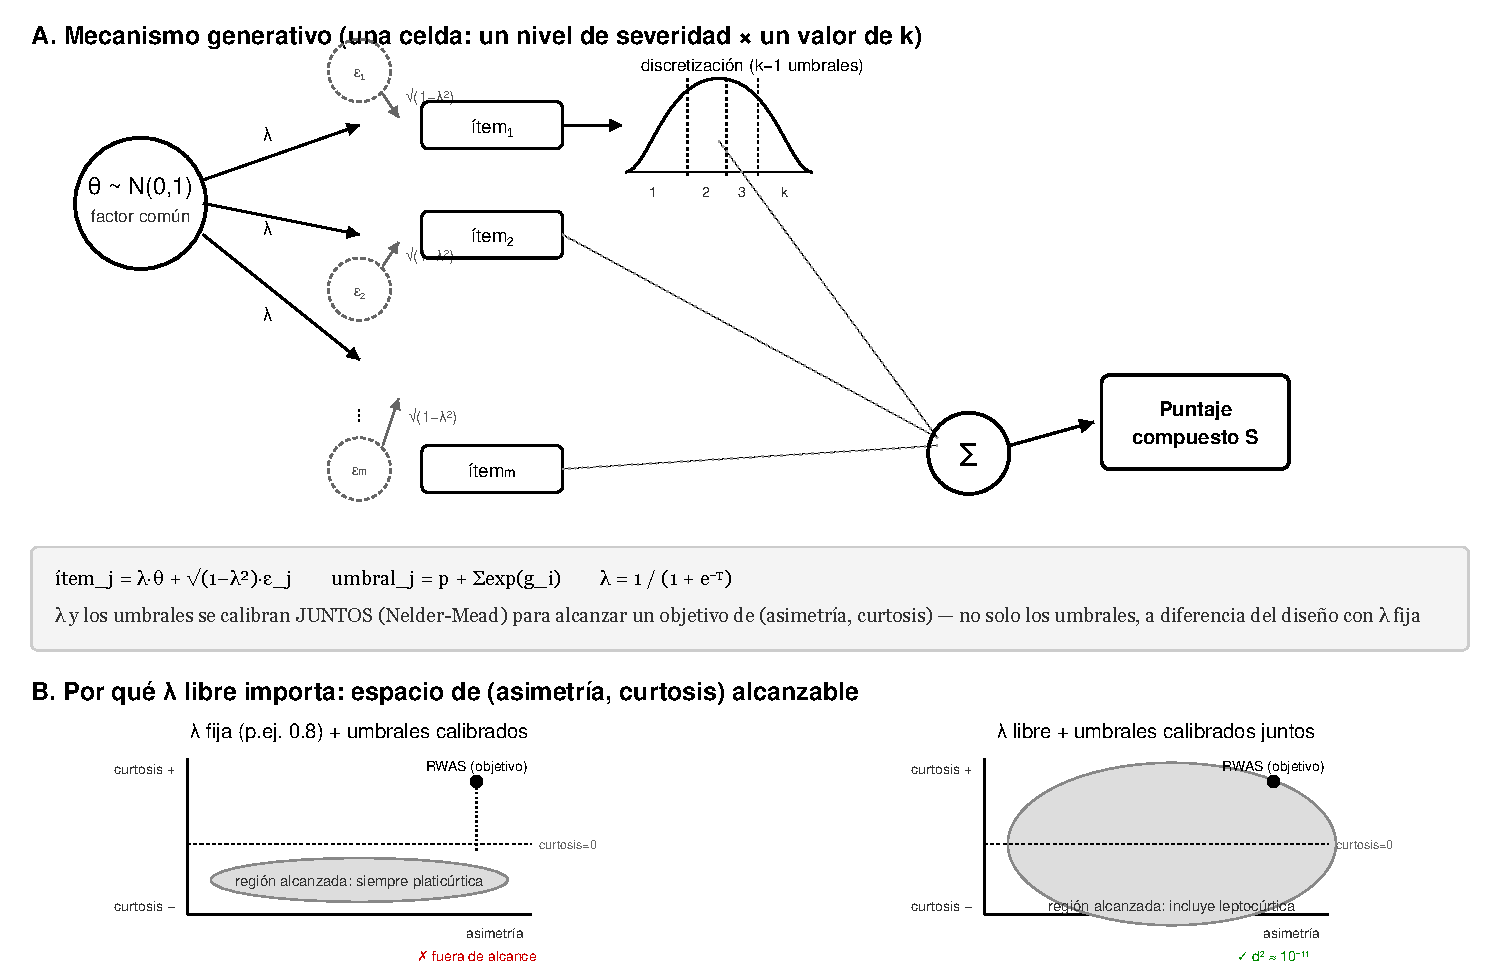
\includegraphics[width=\linewidth]{figuras/mecanismo_lambda_libre.pdf}
\caption{Generative mechanism of the severity-levels block and the skewness/kurtosis space reachable with fixed $\lambda$ versus free $\lambda$}
\label{fig:mecanismo}
\end{figure}

Five ordered levels of non-normality severity were defined, with target skewness and excess kurtosis anchored to the 5th, 25th, 50th, 75th, and 90th percentiles of the 1,567 univariate distributions reported by \textcite{cain2017} (Table~\ref{tab:niveles}). The 90th percentile was used instead of the 95th because the latter proved unreachable in a non-degenerate way with the $m=10$-item mechanism. Kurtosis uses the signed percentile (its direction implies distinct forms of non-normality); skewness uses the percentile of $|\text{skewness}|$, because the power of the 11 tests is symmetric with respect to its direction. Because \citeauthor{cain2017} do not publish absolute-value skewness percentiles nor the 90th percentile, these were derived by linear interpolation of the cumulative distribution function implicit in their table, solving $P(|\text{skewness}| \leq m) = F(m) - F(-m) = p$; this is an approximation over aggregated data, not a calculation over the individual distributions. The skewness and kurtosis percentiles used as targets are marginal, not joint: \citeauthor{cain2017} do not report which combinations of the two co-occur, so each level is a synthetic profile, not an empirical profile jointly observed in psychological practice.

\begin{table}[H]
\small
\caption{Non-normality severity levels and their calibration targets, anchored to percentiles from Cain et al. (2017)}
\label{tab:niveles}
\begin{tabular}{l c >{\centering\arraybackslash}p{3.1cm} >{\centering\arraybackslash}p{3.3cm}}
\toprule
Level & Percentile & \multicolumn{2}{c}{Target} \\
& & Skewness ($|\text{value}|$, interpolated) & Excess kurtosis (signed, direct) \\
\midrule
low & 5th & 0.053 & $-1.28$ \\
low-moderate & 25th & 0.276 & $-0.57$ \\
moderate & 50th (median) & 0.688 & 0.07 \\
high & 75th & 1.332 & 1.62 \\
very high & 90th & 2.401 & 7.52 \\
\bottomrule
\end{tabular}
\tablenote{Level labels (low, low-moderate, moderate, high, very high) are used consistently throughout Results and Discussion.}
\end{table}

\textbf{Calibration.} For each level-by-$k$ combination (seven values, 3 to 9; 35 cells in total), $\lambda$ and the $k-1$ thresholds were calibrated simultaneously via numerical optimization, minimizing the squared distance between the empirical moments of the simulated composite and the targets in Table~\ref{tab:niveles}:

\begin{equation}
d^2 = (\text{skewness}_{\text{achieved}} - \text{skewness}_{\text{target}})^2 + (\text{kurtosis}_{\text{achieved}} - \text{kurtosis}_{\text{target}})^2
\end{equation}

Thresholds were parameterized as $u_1 = p$ and $u_j = p + \sum_{i=2}^{j} \exp(g_i)$, which guarantees increasing thresholds, and $\lambda = 1/(1+e^{-z})$, which keeps it in $(0,1)$. The vector $(z, p, g_1, \ldots, g_{k-2})$ was optimized with Nelder-Mead from 16 starting points per cell, keeping the one with the smallest $d^2$. Moments were computed over $N=150,000$ replications using common random numbers, reused across the 35 cells, so that Monte Carlo noise would not contaminate comparisons between cells.

With the calibrated parameters, each cell (level $\times$ $k$) was simulated independently across the full $n$ grid, with $R=10,000$ replications per cell (280 cells: 5 levels $\times$ 7 values of $k$ $\times$ 8 sample sizes).

\subsection{Real-Data Block: \emph{m-out-of-N} Random Subsampling}
\label{sec:realdata}

On each instrument, repeated random subsampling without replacement was applied, from the \emph{m-out-of-N} family \parencite{politisromanowolf1999} but used here as a Monte Carlo procedure, not with its original asymptotic apparatus: for each $n$ in the grid, $R=10,000$ subsamples were drawn from the instrument's full composite score, and the empirical rejection rate of each test was computed against the full $N$ as the reference population. The minimum $N$ among five of the six instruments (RWAS, 9,680) is far larger than the maximum $n$ in the grid (1,500), so subsampling without replacement is valid for those five without adjustment. The exception is the Adult Hope Scale ($N=1,036$): because it does not reach $n=1,500$, a reduced grid $\{10, 25, 50, 100, 250, 500, 1000\}$ was used only for this instrument. At $n=1,000$ its subsample covers $\sim$97\% of $N$ (vs.\ $\sim$3\% for RSE): there, AHS is not strictly comparable, owing to lower subsampling variability as it approaches a census.

In this component $k$ is not manipulated: it is inherent to each instrument's design, intertwined with its number of items and its real skewness/kurtosis ---as occurs in applied psychometric practice---. The number of items is not varied in any component: constant ($m=10$) in the severity-levels block, specific to each instrument in the real-data block. The severity-levels block exists precisely to isolate $k$ from severity, something the real data do not allow.

\subsection{Normality Tests Evaluated}
\label{sec:tests}

The following battery of 11 normality tests was evaluated: Shapiro-Wilk \parencite{shapirowilk1965}, Anderson-Darling \parencite{andersondarling1954}, Lilliefors \parencite{lilliefors1967}, Jarque-Bera \parencite{jarquebera1980}, D'Agostino-Pearson \parencite{dagostinopearson1973}, Cramér-von Mises \parencite{csorgofaraway1996}, Shapiro-Francia \parencite{shapirofrancia1972}, Pearson's $\chi^2$ \parencite{pearson1900}, the Anscombe-Glynn kurtosis test \parencite{anscombeglynn1983}, Epps-Pulley \parencite{eppspulley1983}, and the SSTN \parencite{anaratschwender2026} ---a recent normality test based on self-similarity under convolution---. None of the 11 plays a leading role in this study: the object of study is the effect of $k$, $n$, and the severity of non-normality on the comparative power of the full battery, not the relative performance of any single test.

\subsection{Implementation and Reproducibility}
\label{sec:implementation}

All simulations and subsampling were run in R (v4.6.1) via GitHub Actions (ubuntu-latest \emph{runners}, one job per cell); the code is available as indicated in Data and Code Availability. With $R=10,000$, the Monte Carlo error of a rate near $.5$ is $\approx.005$; differences smaller than that margin are not systematic. The exact implementation of each test and the category occupancy per cell are documented in the repository (16 of 42 cells --the 35 of the design plus 7 reference cells, one per $k$, Results-- have at least one category with probability $<1\%$).

\subsection{Correction for Decision-Threshold Miscalibration}
\label{sec:correccion}

The nominal criterion ($p<.05$) does not guarantee a 5\% rejection rate under H0 with discrete data. For each test and cell ($k$, $n$), the empirical 5th percentile of $p$-values was calibrated under a reference cell that is equally discrete but has no severity (skewness$=$kurtosis$=0$, not a continuous normal), and the 35 simulated cells and the real subsampling were repeated with that threshold instead of $p<.05$ (same seed). This \emph{corrected power} is size-adjusted to that reference DGP, not power against mathematical normality; the thresholds are specific to each (test, $k$, $n$), not a universal significance level for other scales. It is the primary measure used from here on; the nominal rate serves only as a contrast.

\section{Results}
\label{sec:results}

\subsection{Severity-Levels Block: Effect of \texorpdfstring{$k$}{k}, \texorpdfstring{$n$}{n}, and Non-Normality Severity}
\label{sec:res-niveles}

\begin{enumerate}
\item \textbf{Effect of $k$, nominal criterion.} With $p<.05$, power declines slightly as $k$ increases: the gap (power at $k=3$ minus $k=9$) ranges from .012 to .045 (Table~\ref{tab:brecha-k}).
\item \textbf{The nominal criterion is miscalibrated.} Under the reference cell with no severity, 8 of the 11 tests reject up to 100\% of the time at small $k$ and large $n$ (see the Calibration section below): they detect the discreteness of the composite, not severity. Correcting the decision threshold for this miscalibration (Method), the $k=3-k=9$ gap \textbf{reverses}: from $-.15$ to $-.37$ across the 5 levels (Table~\ref{tab:brecha-k}) --size-adjusted power is higher at $k=9$ than at $k=3$, not lower--.
\item \textbf{Interaction with $n$.} The corrected gap tends to grow in magnitude with $n$, without stabilizing at zero as the nominal gap does (Table~\ref{tab:brecha-n-nivel} and Figure~\ref{fig:brecha}); the trend is not monotonic (there are isolated reversals by level, in addition to the local minimum at $k=7$ within the $k=3$ to $9$ range), but the extremes consistently favor $k=9$ across the 5 levels.
\end{enumerate}

\begin{table}[H]
\small
\caption{Mean power gap between $k=3$ and $k=9$, by severity level (averaged over the 8 sample sizes): nominal vs.\ corrected for miscalibration}
\label{tab:brecha-k}
\begin{tabular}{lcc}
\toprule
Level & Nominal gap & Corrected gap \\
\midrule
low & .027 & $-.322$ \\
low-moderate & .045 & $-.312$ \\
moderate & .036 & $-.365$ \\
high & .016 & $-.199$ \\
very high & .012 & $-.149$ \\
\bottomrule
\end{tabular}
\tablenote{Skewness/kurtosis targets by level in Table~\ref{tab:niveles}.}
\end{table}

\begin{table}[H]
\caption{Corrected power gap between $k=3$ and $k=9$ by severity level and sample size}
\label{tab:brecha-n-nivel}
\begin{tabular}{lccccc}
\toprule
$n$ & low & low-moderate & moderate & high & very high \\
\midrule
10 & $-.048$ & $-.028$ & $-.050$ & $-.108$ & $-.058$ \\
25 & $-.135$ & $-.037$ & $-.102$ & $-.202$ & $-.020$ \\
50 & $-.270$ & $-.061$ & $-.211$ & $-.203$ & $-.045$ \\
100 & $-.371$ & $-.116$ & $-.429$ & $-.077$ & $-.051$ \\
250 & $-.431$ & $-.419$ & $-.580$ & $-.095$ & $-.107$ \\
500 & $-.416$ & $-.574$ & $-.579$ & $-.182$ & $-.182$ \\
1000 & $-.455$ & $-.629$ & $-.524$ & $-.364$ & $-.364$ \\
1500 & $-.454$ & $-.632$ & $-.448$ & $-.364$ & $-.364$ \\
\bottomrule
\end{tabular}
\end{table}

\begin{figure}[H]
\centering
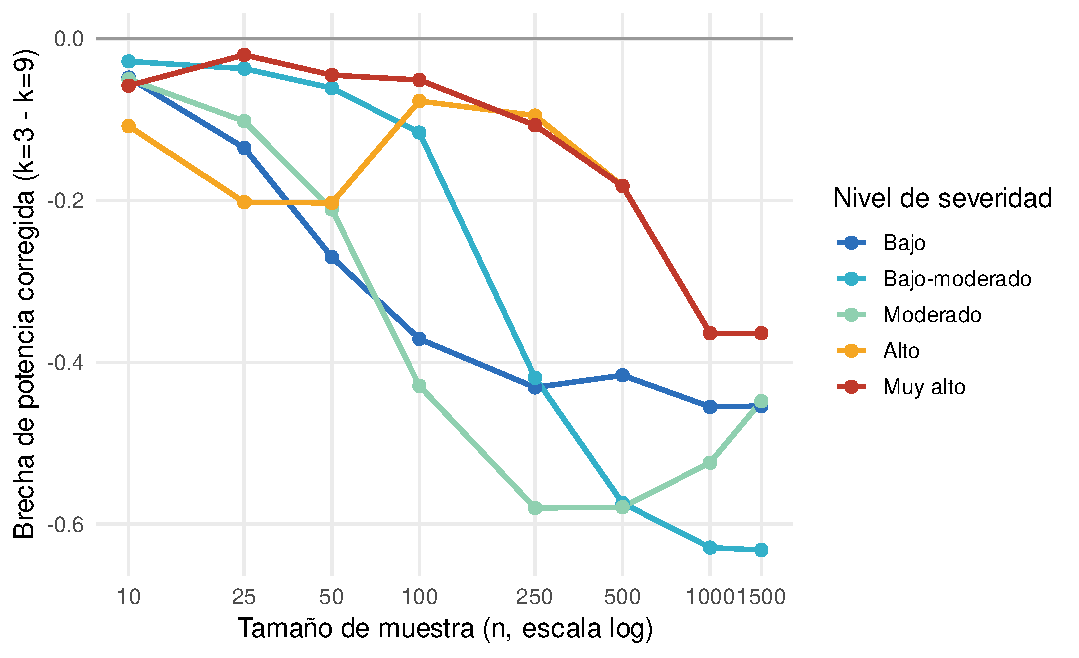
\includegraphics[width=\linewidth]{figuras/brecha_k3_k9_por_n_y_nivel.pdf}
\caption{Corrected power gap between $k=3$ and $k=9$, by sample size and severity level}
\label{fig:brecha}
\end{figure}

\subsection{Calibration of the 11 Tests With No Injected Severity}
\label{sec:res-tipo1}

To separate size-adjusted power from miscalibration, an additional reference cell was simulated (skewness$=$kurtosis$=0$, same discrete mechanism, same $k$ and $n$; not a sixth level, but a reference point) and the empirical rejection rate of each test was measured under that reference DGP. Eight of the 11 tests reject up to 100\% of the time at some point in the grid (Shapiro-Wilk, Anderson-Darling, Lilliefors, Cramér-von Mises, Shapiro-Francia, and Pearson $\chi^2$, at $k=3$, $n=250$; Epps-Pulley and SSTN, at $k=3$, $n=1000$): at small $k$ and large $n$ they detect the discreteness of the composite, not a real deviation in the two moments calibrated to zero here. Jarque-Bera (max $.028$), D'Agostino-Pearson ($.053$), and kurtosis ($.079$) are the three with the smallest maximum deviation from the nominal 5\% across the grid --the rest exceed it by an order of magnitude--. The power reported for the other six tests, especially at small $k$ and large $n$, is therefore entangled with this tendency to reject due to discreteness, not only with the simulated severity.

\subsection{Real-Data Block: Power by Instrument}
\label{sec:res-real}

In this block the true H0 of each instrument is unknown: the \emph{corrected} figure is the rejection rate under the threshold calibrated in the simulated block (Method), not power in the strict sense, and not a size calibration specific to each instrument's number of items (Limitations).

\begin{enumerate}
\item The \emph{nominal} mean rate increases sharply with $n$ and reaches 1.000 for nearly all instruments by $n=500$--$1000$, reproducing the problem seen in the simulated block; but the rate under the calibrated threshold is not necessarily monotonic (next point): RSE and HEXACO ($k=4,7$) plateau at $\approx.27$--$.28$ (Table~\ref{tab:potencia-instrumento}).
\item MACH-IV ($k=5$) and AHS ($k=8$) retain more corrected rate ($\approx.80$--$.88$ at large $n$) than RSE/HEXACO, and RWAS ($k=9$) changes little between nominal and corrected at most $n$ (next point). The pattern is descriptively consistent, across these six instruments, with the reversal seen in the simulated block (not an independent replication of the effect of $k$, above).
\item Recalibrating to the native $m$ of MACH-IV (20), AHS (8), and RWAS (22): MACH-IV's corrected rate drops .05--.10 at $n\geq250$, and RWAS's drops to .91 at $n=1500$; AHS ($m=8$) changes little. $m$ also alters the discrete distribution of the composite and the empirical distribution of $p$ under the reference DGP: the threshold calibrated at $m=10$ is not fully transportable to other $m$.
\item SPS-10 and AHS are not monotonic in $n$: the corrected rate drops from .996 to .909 (SPS-10, $n=500\to1000$) and from .876 to .821 (AHS, $n=500\to1000$); at $n=1000$, AHS is $\approx$97\% of its $N$, but that does not explain SPS-10's drop ($N=91,658$).
\item Assigning each instrument to its nearest simulated level (Euclidean distance in skewness/kurtosis, using $|\text{skewness}|$), RSE, MACH-IV, and HEXACO fall under low-moderate, AHS under moderate, and SPS-10 and RWAS under high.
\end{enumerate}

\begin{table}[H]
\caption{Mean rejection rate (11 tests) by real instrument and sample size: nominal vs.\ \emph{corrected} for miscalibration}
\label{tab:potencia-instrumento}
\begin{tabular}{lcccccccc}
\toprule
Instrument ($k$) & 10 & 25 & 50 & 100 & 250 & 500 & 1000 & 1500 \\
\midrule
RSE (4) nom. & .048 & .063 & .108 & .248 & .719 & .983 & 1.000 & 1.000 \\
RSE (4) corr. & .023 & .037 & .064 & .143 & .265 & .276 & .276 & .275 \\
MACH-IV (5) nom. & .052 & .076 & .131 & .282 & .760 & .989 & 1.000 & 1.000 \\
MACH-IV (5) corr. & .038 & .065 & .121 & .266 & .587 & .733 & .797 & .822 \\
SPS-10 (6) nom. & .158 & .390 & .691 & .924 & .991 & .999 & 1.000 & 1.000 \\
SPS-10 (6) corr. & .134 & .352 & .622 & .844 & .946 & .996 & .909 & .909 \\
HEXACO (7) nom. & .049 & .068 & .104 & .212 & .644 & .967 & 1.000 & 1.000 \\
HEXACO (7) corr. & .020 & .035 & .053 & .121 & .249 & .272 & .273 & .273 \\
AHS (8) nom. & .099 & .217 & .434 & .750 & .919 & .929 & .961 & --- \\
AHS (8) corr. & .074 & .185 & .369 & .588 & .819 & .876 & .821 & --- \\
RWAS (9) nom. & .364 & .749 & .928 & .954 & .984 & .998 & 1.000 & 1.000 \\
RWAS (9) corr. & .349 & .742 & .932 & .961 & .990 & .999 & 1.000 & 1.000 \\
\bottomrule
\end{tabular}
\tablenote{AHS has no $n=1500$ cell because its native $N$ (1,036) does not reach that subsample size without replacement (see Method).}
\end{table}

\subsection{Agreement Between the Calibrated Levels and the 6 Real Instruments}
\label{sec:res-validacion}

The observed power of each instrument was compared with that of its assigned simulated cell (same $k$, nearest level), $n$ by $n$ (Table~\ref{tab:validacion}).

\begin{enumerate}
\item Across the 47 combined cells, $r=.981$; by instrument, $r \geq .957$. Controlling for $n$ (partial correlation), it remains high ($r=.968$). Mean absolute error is .042 (RMSE $=.079$), with a small bias: the simulation overestimates the real rate by .026. Excluding the AHS cell with the largest sampling fraction, or the instrument entirely, does not change this ($r=.981$; RMSE $=.079$–$.085$). These cells share instrument and are not independent; with the \emph{corrected} rate, agreement holds ($r=.977$; partial $r=.972$; RMSE $=.080$); aggregating first by instrument ($N=6$) gives a similar value ($r=.980$), without depending solely on repeated cells.
\item The targets come from an external source \parencite{cain2017}, not from the validation instruments; even so, both use the same coordinates (skewness, kurtosis), so the agreement is not fully independent.
\item Fit distance (0.066--0.450) is moderately associated with prediction error (Spearman $\rho=.37$): the calibration generalizes without a near-perfect fit. This distance sums squared skewness and kurtosis without standardizing, implicitly weighting kurtosis more heavily (larger target magnitude, Table~\ref{tab:niveles}): it is an ad hoc metric, not a neutral one.
\end{enumerate}

\begin{table}[H]
\small
\caption{Correlation and absolute error between real rejection rate and simulated power, by instrument}
\label{tab:validacion}
\begin{tabular}{l l >{\centering\arraybackslash}p{2.1cm} >{\centering\arraybackslash}p{2.1cm} >{\centering\arraybackslash}p{2.1cm}}
\toprule
Instrument ($k$) & Assigned level & Fit distance & $r$ (real vs.\ simulated) & Mean absolute error \\
\midrule
RSE (4) & low-moderate & 0.299 & .986 & .058 \\
MACH-IV (5) & low-moderate & 0.162 & .999 & .015 \\
SPS-10 (6) & high & 0.387 & .957 & .092 \\
HEXACO (7) & low-moderate & 0.066 & .994 & .034 \\
AHS (8) & moderate & 0.273 & .999 & .021 \\
RWAS (9) & high & 0.450 & .995 & .027 \\
\bottomrule
\end{tabular}
\end{table}

\subsection{Simulated-Block Patterns in Real Data}
\label{sec:res-patrones}

The patterns tested do not come from prior literature, which does not cover this cross of factors, nor were they preregistered: they arise from the \emph{corrected} simulated levels block, and here we examine whether they reproduce in the six real instruments, likewise using the corrected rate. Coefficients are estimated by linear regression of power on $k$ (or on the parity of $k$), treating the 11 tests as pseudo-replicates within each assigned severity level --they share the same sample, they are not independent--. They are therefore reported only as a description of the pattern, without their $p$-values, not as inferential evidence.

\begin{description}
\item[More categories ($k$), more corrected rate.] Reproduces under high severity (SPS-10, RWAS): the descriptive coefficient of $k$ was positive at $n=10,25,50$. Under low-moderate (RSE, MACH-IV, HEXACO) it was negative across all 8 sample sizes, because HEXACO ($k=7$) has a corrected rate as low ($\approx.27$) as RSE's ($k=4$) despite having more categories: this coincides with the local minimum at $k=7$ in the simulated block (Discussion).
\item[The effect depends on $n$.] Reproduces: the association with $n$ is descriptively consistent with the simulation: the corrected gap between instruments with different $k$ tends to grow with $n$ rather than shrink.
\item[The gap between extreme $k$ values shrinks with severity.] Cannot be evaluated in the real data: only low-moderate includes several values of $k$; moderate is represented only by AHS.
\item[The parity of $k$ affects power.] No descriptive support: coefficient near zero at $n=10,25,50$.
\end{description}

\subsection{Comparison of the 11 Tests Under the Adjusted Threshold}
\label{sec:res-comparacion}

The mean value under the adjusted threshold of the 11 tests was compared across three scenarios (Table~\ref{tab:ranking}): clean simulated (280 cells, severity isolated from $k$), real (six instruments, rejection rate), and interleaved simulated (same six level-$k$ combinations as the real instruments).

\begin{table}[H]
\small
\caption{Mean value under the adjusted threshold of the 11 tests across the three scenarios, ordered from highest to lowest in the clean simulation}
\label{tab:ranking}
\begin{tabular}{lccc}
\toprule
Test & Clean sim. & Real & Interleaved sim. \\
\midrule
D'Agostino-Pearson & .861 & .775 & .788 \\
Jarque-Bera & .745 & .661 & .685 \\
Shapiro-Wilk & .723 & .491 & .549 \\
Shapiro-Francia & .696 & .474 & .529 \\
Epps-Pulley & .640 & .443 & .502 \\
Kurtosis (Anscombe-Glynn) & .632 & .604 & .561 \\
Anderson-Darling & .560 & .437 & .473 \\
Lilliefors & .491 & .350 & .393 \\
Cramér-von Mises & .482 & .408 & .421 \\
SSTN & .473 & .418 & .420 \\
Pearson $\chi^2$ & .451 & .290 & .339 \\
\bottomrule
\end{tabular}
\end{table}

\begin{itemize}
\item \textbf{D'Agostino-Pearson} has the highest mean value under the adjusted threshold across all three scenarios, and is one of only three tests with the smallest deviation from the nominal 5\% under the reference DGP (\textbf{Jarque-Bera} follows).
\item Corrected, \textbf{Shapiro-Wilk} and \textbf{Shapiro-Francia} retain a considerable value (.49--.72) despite being poorly calibrated: miscalibration inflated their \emph{nominal} power, without rendering them useless.
\item \textbf{Pearson $\chi^2$} has the lowest mean value of the 11 across the three aggregated scenarios --not necessarily in every individual combination of $k$, $n$, and severity-- and is poorly calibrated.
\item The mean ordering is consistent across scenarios, compatible with using the clean simulation as a controlled comparative reference among tests.
\end{itemize}

\section{Discussion}
\label{sec:discussion}

The study shows a systematic association between response categories and the power of normality tests, but the nominal criterion ($p<.05$) describes it backwards from what actually occurs. Under that criterion, power declines slightly as $k$ increases (gap of .012 to .045). But 8 of the 11 tests reject up to 100\% of the time under the reference cell with no severity (Method) when $k$ is small and $n$ is large --they detect the discreteness of the composite, not severity--, so much of that nominal power is miscalibration, not detection. Correcting the decision threshold for that miscalibration, the gap reverses and tends to grow with $n$ rather than shrink (from $-.15$ to $-.37$ across the 5 levels): size-adjusted power relative to that reference DGP is higher at large $k$ than at small $k$, although not in a perfectly monotonic way (below). This adds a further consideration, alongside those already known regarding reliability and validity \parencite{lozano2008,preston2000}, for weighing the consequences of using scales with very few categories: with few categories, the interpretation of these tests can be seriously compromised by the miscalibration induced by the discreteness of the composite.

The relationship is not perfectly monotonic between $k=3$ and $9$: there is a local minimum at $k=7$, in several simulated levels and replicated in HEXACO (the only real instrument with that $k$), not explained by worse calibration or by $\lambda$ --possibly because equating only two moments does not uniquely fix the complete shape of the distribution, with no causal identification--. Even so, the extremes favor large $k$ across the 5 simulated levels and, descriptively, across the six real instruments (Results).

A further source of heterogeneity in the real data is composition by country and sex: the $N$ mixes populations without checking invariance. Two post hoc checks ($n=250$; chi-square test of homogeneity of proportions, Bonferroni for 55 comparisons $=5$ instruments $\times$ 11 tests) detect differences concentrated in MACH-IV and RSE, with greater magnitude by sex (Cohen's $w=0.13$–$0.48$) than by country ($w=0.11$–$0.43$); SPS-10, RWAS (and AHS by sex) remain saturated. Repeating both with the \emph{corrected} rate --descriptive, not an inferential contrast-- RSE's difference shrinks substantially --it was mostly miscalibration--, while MACH-IV's difference by sex barely attenuates: consistent with documented sex differences in Machiavellianism \parencite{muris2017,confino2024}, whereas in self-esteem sex differences are also documented, generally small \parencite{kling1999}. This post hoc agreement does not constitute an independent validation of the method.

Among the tests, D'Agostino-Pearson and Jarque-Bera combine the highest mean values under the adjusted threshold with the smallest deviation from the nominal 5\%; Shapiro-Wilk and Shapiro-Francia retain a considerable value under the adjusted threshold despite being poorly calibrated, so using them requires correcting the threshold, not discarding them; Pearson $\chi^2$ has the lowest mean value across the three scenarios.

Limitations include a composite of 10 items with a single common factor --recalibrated to the native $m$ for only 3 of 6 instruments (Results)--, one real instrument per value of $k$ (with SPS-10 non-monotonic in $n$), and that the parity of $k$ and the trend of the gap with severity could not be evaluated in real data. The six instruments are not replicates of a common design: this is an illustration of transportability, not generalizable beyond these six cases. The calibration equates only skewness and kurtosis, not the complete distributional shape: the effect attributed to $k$ is defined under this specific family of DGPs, not as a general property. The $k=7$ anomaly remains without a causal explanation. The results apply to composite scores, not to individual items.

\section*{Data and Code Availability}
The generated data and the complete code (extraction, calibration, simulation, subsampling, analysis and aggregation, and GitHub Actions configuration) are available at \blindtext{\url{https://github.com/ArchieJamDev/ResponseCategories-Normality-Study}}{an anonymized mirror of the repository (identifying information removed for double-blind review; the original link is restored after acceptance)}. The raw data for the six instruments are available at the sources cited in the Method. The study was not preregistered.

\section*{Use of Generative Artificial Intelligence}
Generative artificial intelligence (Claude, Anthropic) was used to implement and run the R code and as a writing assistant, always under the author's review and direction; the author made all conceptual and methodological decisions.

\section*{Declarations}

\textbf{Funding.} The author received no specific funding for this work.

\textbf{Conflict of Interest.} The author declares no conflicts of interest.

\textbf{Ethical Approval.} Not applicable. No new data were collected from human participants; all real-data examples reuse previously published, publicly available, and de-identified datasets (see Real Psychometric Instruments in the Method, and the Data Availability statement above).

\textbf{Consent to Participate and for Publication.} Not applicable.

\textbf{Author Contribution.} Single-authored manuscript; A.C. conceived the study, designed and executed the analyses, and wrote the manuscript.

\printbibliography

\end{document}
